\subsection{Three-direction warm-up and recovery}\label{app:recoveryhistory}
Reconstruction warm-up makes 40 passes through 392,000 patches, with 191
complete batches of 2,048 per epoch. Adam uses the released OneCycle schedule
(maximum learning rate 0.003, 5\% warm-up). The checkpoint with lowest
development mean squared error (MSE) starts guided training: 2,500 eight-image
updates, Adam at $3\times10^{-4}$, gradient-norm clipping at 5, and noise
scaled by 0.1. Reconstruction, contrast, and detection receive weights
$1$, $0.05$, and $0.01$. Checkpoints are evaluated every 250 updates against
the unchanged MSE limit from the common native reference, trained on
reconstruction alone. Endpoints that fail this limit remain in the evaluation records.

Recovery run \texttt{766a3dfee0e3} continues the guided endpoint and trained
heads for 500 updates, either with the original loss or with fourfold
reconstruction weight. Both arms reset Adam, match image/noise streams,
fix assignments, and evaluate every 50 updates. Native references and SVD
initialization are reused. After inspecting recovery, we chose the ordinary-loss
endpoint at update 500 for every run. This choice uses the
same endpoint rule across seeds, rather than selecting the best checkpoints
or separate arms. It gives 3,000 guided updates after reconstruction warm-up.

Table~\ref{tab:recovery-arms} uses the reused 1,500-image test and calibration-selected
readouts. Neither continuation meets the native-reference MSE limit in any
seed. The mask-initialized fallback meets that limit. That fallback
is a different checkpoint from the continuation endpoints.
\begin{table*}[t]\centering\small
\caption{Mean $\pm$ sample SD. Recovery-arm means on the reused test. Only the mask-initialized fallback meets the native MSE rule.}\label{tab:recovery-arms}
\begin{tabular}{@{}lrrr@{}}\toprule
State & Capture & AP & VE\\\midrule
Ordinary continuation & $33.32\pm0.31$ & $75.06\pm0.26$ & $64.50\pm0.08$\\
$4\times$ reconstruction & $31.88\pm0.24$ & $74.49\pm0.22$ & $64.57\pm0.08$\\
Mask-initialized fallback & $26.88\pm0.08$ & $71.40\pm0.69$ & $65.10\pm0.06$\\
\bottomrule\end{tabular}

\end{table*}

\subsection{Random-initialized continuation with three-direction groups}\label{app:earlierprotocol}
\paragraph{Native training.}
Each epoch shuffles patches into complete batches and drops the remainder.
Adam uses its default momentum settings, and OneCycleLR steps after every
update with maximum learning rate 0.003, 5\% warm-up, cosine annealing, and
division factors 25 and $10^4$. Validation runs every 500 updates and at the
end. Seeds 21 and 22 select update 7,640, while seed 23 selects 7,500.
All random-initialized runs consume 7,640 updates without masks for fitting
or selection. Mask warm-up also has no mask loss, but begins with mask-derived weights.

\paragraph{Matched continuation.}
Both arms share selected native weights, fresh Adam, and paired image/noise
streams seeded by $71{,}000+\mathrm{dictionarySeed}$. Updates sample eight
images with replacement ($8\times196$ patches), use learning rate 0.0003,
clip gradient norm at 5, and renormalize decoder directions. All selection
images are scored every 250 updates. Core parameters total
$2dGr+Gr=4,721,664$, without decoder bias. Detection adds 150 training-only
parameters.

Readout selection uses all 2,000 training images and requires minimum category
evidence. Contrast readouts maximize pooled error reduction under the existing
decoder, while detector readouts maximize non-interpolated AP. Assignments
remain fixed for 2,500 updates but may be shared across categories or differ
between metrics. Negative-only detection pools remain valid.

\paragraph{Checkpoint selection.}
The 2\% limit uses common native-start development MSE. Object-score selection
includes update zero and selects the checkpoint with fewer updates when scores tie
(Table~\ref{tab:selected-updates}). Training or test loss cannot replace this reference.

Every arm receives 2,500 updates, and a separate evaluation of the
minimum-MSE continuation checkpoint is retained.

\begin{agfresulttable}
\caption{Random-initialized GGF minus matched continuation: Capture gains and paired image intervals.}\label{tab:guided-seed-gains}
\begin{tabular}{@{}lrr@{}}
\toprule
Seed & Gain (pp) & 95\% interval \\
\midrule
21 & 9.75 & [9.43, 10.01] \\
22 & 10.55 & [10.25, 10.91] \\
23 & 9.95 & [9.74, 10.24] \\
\bottomrule
\end{tabular}

\end{agfresulttable}

\subsection{Complete per-start results and loss ablation}\label{app:ablation}
\begin{figure}[htbp]\centering
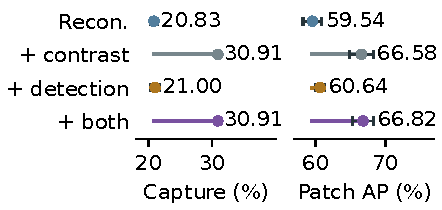
\includegraphics[width=175bp]{figures/agf_loss_lollipop.pdf}
\caption{Three-direction loss ablation from random initialization:
means with sample-SD error bars on a separate inspected holdout. Every arm
retains reconstruction. Lines show changes from reconstruction-only
continuation. Numbers are percentages.}\label{fig:loss-ablation-main}\label{fig:guided}\label{fig:guided-detail}
\end{figure}


The loss ablation uses random initialization and fixed group membership.
The three-direction mask-initialized checkpoints are evaluated separately in Appendix~\ref{app:matched-baselines}.
\begin{agfresulttable}
\caption{Random-initialized runs and loss-ablation scores on the common test. Scores are percentages, and Update is the selected checkpoint. Rec. only is matched continued Vanilla. Contrast, detection and Both retain reconstruction. Every continued or guided branch consumes 2,500 updates. Selected checkpoints follow the same object-score rule. Final-step scores remain separately recorded.}\label{tab:full}\label{tab:ablationseeds}\label{fig:ablation-summary}\label{tab:selected-updates}
\begin{tabular}{@{}llrrrr@{}}
\toprule
Seed & Loss or state & Update & Capture (\%) & AP (\%) & VE (\%) \\
\midrule
21 & Native & 7640 & 20.80 & 59.57 & 65.39 \\
21 & Rec. only & 1500 & 20.90 & 58.91 & 64.87 \\
21 & + contrast & 2500 & 30.64 & 64.62 & 64.71 \\
21 & + detection & 1250 & 21.12 & 60.16 & 64.89 \\
21 & Both & 2500 & 30.65 & 65.05 & 64.72 \\
22 & Native & 7640 & 20.15 & 61.32 & 65.42 \\
22 & Rec. only & 2000 & 20.25 & 61.08 & 64.86 \\
22 & + contrast & 2500 & 30.79 & 67.56 & 64.80 \\
22 & + detection & 2000 & 20.31 & 61.36 & 64.86 \\
22 & Both & 2500 & 30.80 & 67.61 & 64.80 \\
23 & Native & 7500 & 21.43 & 59.26 & 65.38 \\
23 & Rec. only & 1250 & 21.33 & 58.62 & 64.82 \\
23 & + contrast & 2250 & 31.29 & 67.55 & 64.72 \\
23 & + detection & 2500 & 21.59 & 60.38 & 64.82 \\
23 & Both & 2250 & 31.29 & 67.82 & 64.72 \\
\bottomrule
\end{tabular}

\end{agfresulttable}

Compatible combined/control checkpoints are reused. Environment changes
trigger documented replay from saved native weights, not silent native
retraining. All arms retain reconstruction, fixed assignments, masks, 2,500
updates, noise, and checkpoint rules. Zero-weight losses may be logged.
Detector heads receive no gradient when detection weight is zero.

Contrast alone improves both Capture and AP, whereas detection alone gives
a smaller AP gain and little Capture gain. Contrast is the principal
source of improvement in this setting. Per-category records for the three-direction ablation are included in the
reproducibility materials. Figure~\ref{fig:current-categories} gives
per-category results for the separate 4,096-group, twelve-direction comparison.
\subsection{Loss-weight screen and random-start diagnostic}\label{app:sweep}
The loss-weight screen in Figure~\ref{fig:loss-weight-main} supports retaining
the original weights: doubling detection slightly raises AP with little
change in Capture, whereas reducing or doubling contrast lowers Capture at
the selected checkpoint. This exploratory development comparison does not
establish an optimum.

\begin{agfresultsfigure}
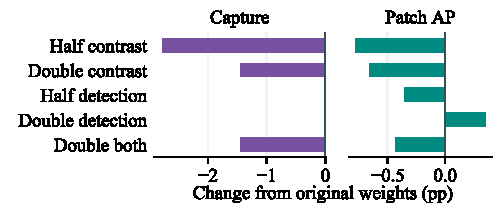
\includegraphics[width=.94\linewidth]{figures/agf_loss_weight_main.pdf}
\captionof{figure}{Loss-weight screen: selected-checkpoint changes from original weights, seed 21, reused development data. Table~\ref{tab:sweep-selected} gives full scores.}\label{fig:loss-weight-main}
\end{agfresultsfigure}

The seed-21 screen uses 2,000 training images and the inspected 400-image
selection set, without accessing test data. Six settings start from identical
native weights and receive 2,500 updates with fresh Adam at 0.0003,
zero-initialized heads, eight-image batches, norm-5 clipping, fixed training
readouts, and paired image/noise streams. Reconstruction weight remains one,
and source and batch hashes verify pairing.
\begin{table*}[t]
\centering
\small
\setlength{\tabcolsep}{3pt}
\renewcommand{\arraystretch}{1.05}
\caption{The development loss-weight screen reports selected checkpoints for seed 21. Capture, Patch AP and VE are percentages. Random start uses a different initialization and less total pretraining computation.}
\label{tab:sweep}\label{tab:sweep-selected}\label{fig:sweep}
\begin{tabular}{@{}lrrrrrr@{}}
\toprule
Setting & \shortstack{Contrast\\weight} & \shortstack{Detection\\weight} & \shortstack{Selected\\update} & Capture (\%) & Patch AP (\%) & VE (\%) \\
\midrule
Original weights & 0.050 & 0.010 & 2500 & 30.08 & 63.34 & 64.66 \\
Half contrast & 0.025 & 0.010 & 2500 & 27.30 & 62.56 & 64.75 \\
Double contrast & 0.100 & 0.010 & 500 & 28.64 & 62.68 & 64.68 \\
Half detection & 0.050 & 0.005 & 2500 & 30.07 & 62.99 & 64.67 \\
Double detection & 0.050 & 0.020 & 2500 & 30.07 & 63.69 & 64.66 \\
Double both & 0.100 & 0.020 & 500 & 28.63 & 62.91 & 64.67 \\
Random start & 0.050 & 0.010 & 2500 & 25.94 & 40.11 & 58.98 \\
\bottomrule
\end{tabular}

\end{table*}
\begin{agfresulttable}
\caption{Mean $\pm$ sample SD. Matched-update loss-ablation means on the inspected holdout.}\label{tab:loss-means}
\begin{tabular}{@{}lrr@{}}\toprule
Losses & Capture & Patch AP\\\midrule
Reconstruction & $20.83\pm0.55$ & $59.54\pm1.34$\\
+ contrast & $30.91\pm0.34$ & $66.58\pm1.69$\\
+ detection & $21.00\pm0.65$ & $60.64\pm0.64$\\
+ both & $30.91\pm0.33$ & $66.82\pm1.54$\\
\bottomrule\end{tabular}

\end{agfresulttable}
Double detection is only 0.0094 Capture points below the original weights.
The screen does not distinguish a unique optimum.

\paragraph{Selected versus final.}
Table~\ref{tab:sweep-rejected} records the higher-Capture but ineligible
endpoints. Both settings fail the 2\% MSE guard at all eight audits from
750 through 2,500, so selection retains update 500. The violation persists
at the endpoint rather than only during an early spike.
\begin{agfresulttable}
\caption{Rejected endpoints and retained update-500 Capture.}\label{tab:sweep-rejected}
\begin{tabular}{@{}lrrr@{}}
\toprule
Weights & Final Capture (\%) & MSE rise (\%) & Retained (\%) \\
\midrule
Double contrast & 32.86 & 2.468 & 28.64 \\
Double both & 32.85 & 2.455 & 28.63 \\
\bottomrule
\end{tabular}

\end{agfresulttable}

\paragraph{No-pretraining diagnostic.}
A random model (seed $104{,}092+21$) receives the original loss and
2,500 guided updates, with 74 unique detector and 69 contrast assignments
(Table~\ref{tab:scratch}). AP peaks at 44.30\% at update 750, then falls
while Capture and VE rise. The cause is untested. Native-start arms also
use 7,640 pretraining updates, so this is not total-compute matched or
evidence that pretraining is necessary.
\begin{agfresulttable}
\caption{Guided training from a random start.}\label{tab:scratch}
\begin{tabular}{@{}lrrr@{}}
\toprule
Model or state & Capture (\%) & AP (\%) & VE (\%) \\
\midrule
Update 0 & 0.55 & 10.70 & 19.31 \\
Update 2,500 & 25.94 & 40.11 & 58.98 \\
\bottomrule
\end{tabular}

\end{agfresulttable}

\paragraph{Selection and limits.}
Checkpoint selection, including update zero, maximizes Capture
$+0.2\,\mathrm{AP}$ within native MSE $\times1.02$. Weight recommendations
instead maximize Capture while keeping AP/VE within 0.1 point and MSE within
2\% of the original-weight control. These engineering margins are not
equivalence tests. None of the six native-start settings dominates another
under the Pareto criterion: at least as good on all three metrics and better
on one. Each comparison uses 200 valid paired image draws without tuning or
multiplicity correction. Original weights gain 0.47 Capture point in their
final 500 updates, so no plateau is established.

